\section{Auswertung}
\label{sec:Auswertung}

\subsection{Fehlerrechnung}
Der Mittelwert eines Datensatzes mit $N$ Werten ist definiert durch:
\begin{equation}
  \bar{x} = \frac{1}{N} \sum_{i=1}^N x_i
\end{equation}
Die Standardabweichung eines Datensatzes von seinem Mittelwert durch:
\begin{equation}
  \sigma = \sqrt{\frac{1}{N(N-1)} \sum_{i=1}^N (x_i - \bar{x})}
\end{equation}
Pflanzen sich Unsicherheiten fort, wird der Fehler mit der gaußschen
Fehlerfortpflanzung berechnet:
\begin{equation}
  \sigma_f = \sqrt{
      \sum\limits_{i = 1}^N
       \left( \frac{\partial f}{\partial x_i} \sigma_i \right)^{\!\! 2}
     }
\end{equation}
Der Fehler der Steigung $m$ und des Achsenabschnittes $b$ einer linearen Regression
wird wie folgt berechnet:
\begin{align}
  \sigma_m &= \frac{\overline{xy}-\bar{x}\cdot\bar{y}}{\bar{x^2}-\bar{x}^2} \\
  \sigma_b &= \frac{\bar{x^2}\bar{y}-\overline{xy}\bar{x}}{\bar{x^2}-\bar{x}^2}
\end{align}


\subsection{Entladevorgang des Kondensators}
In Tabelle 1 sind die gemessenen Spannungen, bei dem Entladevorgang des Kondensators, zu den jeweiligen Zeitpunkten dargestellt. Zudem
ist der Bruch $\frac{U}{U_0}$ tabelliert, welcher für weitere Rechnungen nötig ist. Die Generatorpannung beträgt
dabei $U_0 = 3.30$V.

\begin{table}[H]
  \centering
  \caption{Gemessene Spannungen bei dem Entladen eines Kondensators}
  \label{tab:Rechteckspannung}
  \begin{tabular}{c c c}
    \toprule
    $t/\left(10^{-3}\symup{s}\right)$ & $U_C/$V & $\ln{\frac{U_C}{U_0}}$ \\
    \midrule
    0.5 & 2.36 & -0.33 \\
    1.0 & 1.62 & -0.71 \\
    1.5 & 1.08 & -1.11 \\
    2.0 & 0.72 & -1.51 \\
    2.5 & 0.48 & -1.90 \\
    3.0 & 0.32 & -2.30 \\
    3.5 & 0.18 & -3.00 \\
    4.0 & 0.12 & -3.22 \\
    4.5 & 0.06 & -3.91 \\
    5.0 & 0.04 & -4.61 \\
    \bottomrule
  \end{tabular}
\end{table}

Aus Gleichnung \eqref{eqn:Entladung} folgt:
\begin{equation}
  \ln{\frac{U}{U_0}} = -\frac{1}{RC}t.
\end{equation}
Der Logarithmus von $\frac{U}{U_0}$ wird gegen die Zeit aufgetragen und es wird eine lineare Regression durchgeführt.



\begin{figure}[H]
  \centering
  \includegraphics{plot1.pdf}
  \caption{Logarithmus der Kondensatorspannung zu dem Zeitpunkt t}
  \label{fig:entladung}
\end{figure}

Die Gerade kann durch die Gleichung $y = -\frac{1}{m}x + b$ beschrieben werden. Für die Parameter ergeben sich:
\begin{align*}
  -\frac{1}{m} = &RC = (1.08 \pm 0.04) \, \symup{s} \\
  &b = (0.28 \pm 0.11)
\end{align*}

Der Fehler der Parameter wird mit Gleichung (18) und (19) berechnet.

\subsection{Bestimmung der Zeitkonstante mit frequenzabhängiger Amplitude und Phasenverschiebung}

In Tabelle 2 ist die Amplitude $A$ und Phasenverschiebung für verschiedene Frequenzen dargestellt. Zudem ist der
Abstand der Nulldurchgänge $a$ tabelliert. Die Generatorspannung beträgt $U_0 = 3.60$V.

\begin{table}[H]
  \centering
  \caption{Gemessene Amplituden und Phasenverschiebungen der Kondensatorspannung}
  \label{tab:amplitude}
  \begin{tabular}{c c c c}
    \toprule
    $\omega/$Hz & $A/$V & $a/\left(10^{-3}\symup{s}\right)$ & $\varphi /°$ \\
    \midrule
    30   &  3.40 &    1.00 &  10.80 \\
    70   &  3.00 &    1.20 &  30.24 \\
    100  &  2.68 &    1.20 &  43.20 \\
    300  &  1.24 &    0.60 &  64.80 \\
    700  &  0.56 &    0.31 &  78.12 \\
    1000 &  0.40 &    0.22 &  79.20 \\
    2000 &  0.20 &    0.12 &  86.40 \\
    3000 &  0.13 &    0.08 &  86.40 \\
    4000 &  0.10 &    0.06 &  86.40 \\
    5000 &  0.08 &    0.05 &  90.00 \\
    \bottomrule
  \end{tabular}
\end{table}

Die Spannungsamplitude $\frac{A}{U_0}$ wird gegen $\ln{\omega}$ aufgetragen. Es wird eine nicht lineare
Regression durchgeführt.

\begin{figure}[H]
  \centering
  \includegraphics{plot2.pdf}
  \caption{Amplitude der Kondensatorspannung in Abhängkeit der Frequenz}
  \label{fig:amplitude}
\end{figure}

Als Ausgleichsfunktion wird $f(\omega) = \frac{1}{\sqrt{1 + c^2 \omega^2}}$, welche auf Gleichung (13)
zurückzuführen ist.
Der Parameter $c$ beträgt:
\begin{align*}
  c = RC = \SI{-9.2(1)e-3}{\second}.
\end{align*}

Die Zeitkonstante wird nun mithilfe der Phasenverschiebung bestimmt. Die Phasenverschiebung wird gegen
den Logarithmus der Frequenz aufgetragen. Eine nicht lineare Regression wird gemäß der Gleichung (11) durchgeführt.
Die Ausgleichsfunktion lautet $f(\varphi) = \arctan(d\varphi)$. Das Minuszeichen in der Funktion wird
weggelassen, da das Oszilloskop den Betrag der Phasenverschiebung anzeigt.

\begin{figure}[H]
  \centering
  \includegraphics{plot4.pdf}
  \caption{Phasenverschiebung in Abhängkeit der Frequenz}
  \label{fig:phasenverschiebung}
\end{figure}


Die Spannungsamplitude $\frac{A}{U_0}$ wird gegen $\varphi$ aufgetragen.

\begin{figure}[H]
  \centering
  \includegraphics{plot3.pdf}
  \caption{Polarplot von Amplitude und Phasenverschiebung.}
  \label{fig:Polarplot}
\end{figure}

Die Theoriekurve ergibt sich aus der Gleichung
\begin{equation}
  \frac{A}{U_0} = cos(\varphi)
\end{equation}

\subsection{Nutzung des RC-Kreises als Integrator}

\begin{figure}[H]
  \centering
  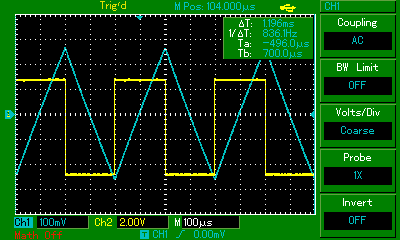
\includegraphics{MAP001.png}
  \caption{Eingang: Rechteckspannung}
  \label{fig:Rechteckspannung}
\end{figure}

Bei einer Rechteckspannung ergibt sich eine Dreieckspannung als integrierte Spannung.

\begin{equation*}
  f(x) =
  \begin{cases}
    a & \text 0 < x < b \\
    -a & \text b < x < 2b \\
  \end{cases}
\end{equation*}
Integriert:
\begin{equation*}
  F(x) =
  \begin{cases}
    a \cdot x & \text 0 < x < b \\
    -a \cdot x & \text b < x < 2b \\
  \end{cases}
\end{equation*}

\begin{figure}[H]
  \centering
  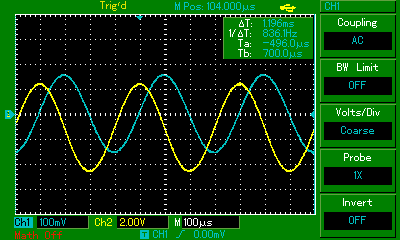
\includegraphics{MAP002.png}
  \caption{Eingang: Sinusspannung }
  \label{fig:Sinusspannung}
\end{figure}

Bei einer Sinusspannung ergibt sich eine Cosinusspannung als integrierte Spannung.
\begin{equation*}
  f(x) = a \cdot sin(x)
\end{equation*}
Integriert:
\begin{equation*}
  F(x) = -a \cdot cos(x)
\end{equation*}

\begin{figure}[H]
  \centering
  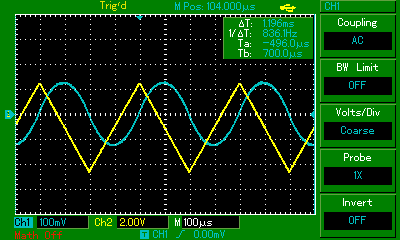
\includegraphics{MAP003.png}
  \caption{Eingang: Dreieckspannung}
  \label{fig:Dreieckspannung}
\end{figure}

Bei einer Dreieckspannung ergibt sich eine quadratische Funktion als integrierte Spannung.
\begin{equation*}
  f(x) =
  \begin{cases}
    a \cdot x & \text 0 < x < b \\
    -a \cdot x & \text b < x < 2b \\
  \end{cases}
\end{equation*}
Integriert:
\begin{equation*}
  F(x) =
  \begin{cases}
    \frac{a}{2} \cdot x^2 & \text 0 < x < b \\
    -\frac{a}{2} \cdot x^2 & \text b < x < 2b \\
  \end{cases}
\end{equation*}
